\subsection{Análisis cualitativo de resultados}

Sumado a la comparación entre distintas implementaciones del
\textsc{Disjoint-Set} en esta sección mostraremos segmentaciones resultantes de
ejecutar el algoritmo con distintos parámetros. También se ofrecen adjuntos
tres videos dónde se varía cada uno de los parámetros mientras se fijan los
otros dos\footnote{Dado que la forma en la que elegimos los colores no resultó
estable respecto de variar $\sigma$ el video dónde se lo varía podría resultar
molesto para personas con fotosensibildad.}.

\subsubsection{Calidad de una segmentación}

Una buena segmentación es un concepto difícil de definir, dado que depende el
nivel de granularidad deseado ciertos segmentos pueden resultar útiles o no
(ventanas en edificios, ojos en personas, letras individuales en una hoja,
etc). Cómo nuestro algoritmo sólo percibe la intensidad de cada píxel se pierde
información propia del color en la transformación que nos genera casos de error
que podrían salvarse de otro modo.

\subsubsection{Segmentación de una imagen con distintas texturas definidas}

Como primer ejemplo construimos una imagen con 3 (o 2) regiones definidas: un
degradé, una región de color sólido y una región con ruido.

\begin{figure}[h]
	\centering
	\begin{subfigure}{0.4\linewidth}
		
\includegraphics[width=\linewidth]{segmentation/entradas-posta/sintetico}
		\caption{Entrada}
	\end{subfigure}
	\begin{subfigure}{0.4\linewidth}
		\includegraphics[width=\linewidth]{segmentation/salidas/{0.8.sintetico.png.500.1000}.png}
		\caption{Segmentación}
	\end{subfigure}
	\caption{$\sigma = 0.8,\ k = 500,\ g = 1000$.}
\end{figure}

El resultado del algoritmo es bueno pero requiere del postproceso de
simplificación para eliminar pequeños segmentos que quedan dentro de la región
con ruido. Una segmentación alternativa válida podría ubicar al degradé y el
color sólido dentro de la misma región, pero dada la definición de $\tau(e)$ y
el orden en el cual se construyen las regiones la región sólida tendrá un valor
de $\tau$ muy pequeño para el momento en el que se evalúen las aristas que la
unen con el degradé.

\subsubsection{Segmentación de una imagen de vida silvestre}

\begin{figure}[h]
	\centering
	\begin{subfigure}{0.4\linewidth}
		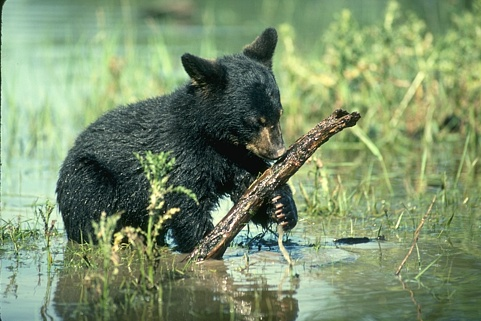
\includegraphics[width=\linewidth]{segmentation/entradas-posta/oso}
		\caption{Entrada}
	\end{subfigure}
	\begin{subfigure}{0.4\linewidth}
		\includegraphics[width=\linewidth]{segmentation/salidas/{0.8.oso.jpg.500.100}.png}
		\caption{Segmentación}
	\end{subfigure}
	\caption{$\sigma = 0.8,\ k = 500,\ g = 100$.}
\end{figure}

En esta segmentación existen varios resultados esperables. De acuerdo a la
granularidad con la que miremos la imagen podemos pensar en distintas
segmentaciones:

\begin{itemize}
	\item \textbf{Granularidad alta:}
		El cuerpo del oso, su nariz, su reflejo, cada planta en la
		foto, la rama, el agua, las uñas del oso.
	\item \textbf{Granularidad baja:}
		El oso, el agua, las plantas, la rama, el agua.
\end{itemize}

En el resultado conseguido podemos ver que se construyó un segmento con la
planta que está por delante del oso pero esta planta está en un segmento
distinto que el resto de las plantas\footnote{Esto será así siempre, dado que
nuestra implementación sólo tiene en cuenta los píxeles inmediatamente vecinos,
por lo que no puede reconocer objetos por sí mismos sino sólo regiones que
mantieneni cierta similaridad interna.} las cuales acabaron en un segmento
grande que podemos interpretar como ``fondo'' de la imagen. Lo mismo que
ocurrió con la planta ocurrió con el oso, que vió su brazo en un segmento
distinto del resto de su cuerpo.

Podemos categorizar a esta segmentación como una de granularida baja.

\newpage

\subsubsection{Segmentación de una imagen con regiones planas}

Finalmente analicemos la segmentación de una imagen con dos objetos claramente
definidos y muchas regiones planas (que pueden o no resultar de interés de
acuerdo al uso requerido).

\begin{figure}[h]
	\centering
	\begin{subfigure}{0.4\linewidth}
		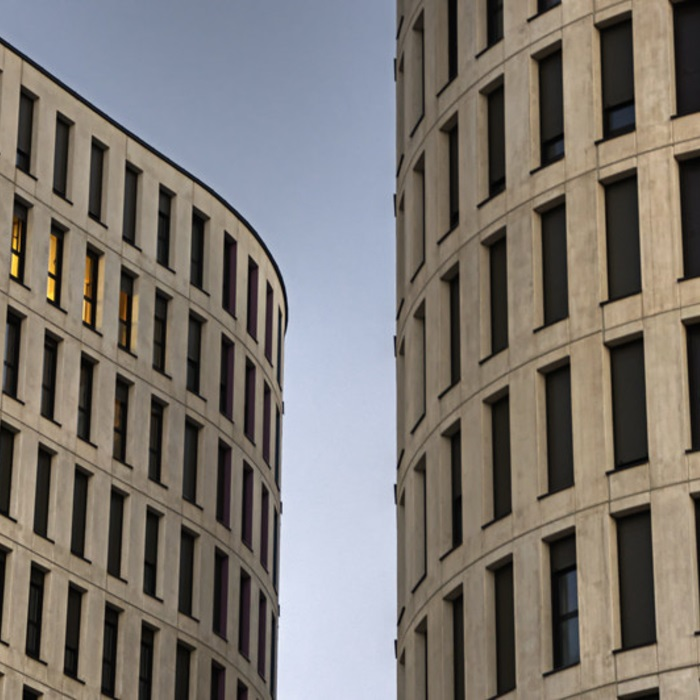
\includegraphics[width=\linewidth]{segmentation/entradas-posta/edificios}
		\caption{Entrada}
	\end{subfigure}
	\begin{subfigure}{0.4\linewidth}
		\includegraphics[width=\linewidth]{segmentation/salidas/{0.8.edificios.png.600.-1}.png}
		\caption{Segmentación}
	\end{subfigure}
	\caption{$\sigma = 0.8,\ k = 600$.}
\end{figure}

En el edificio de la izquierda puede notarse que se tomó casi todo como un
único segmento. Esto puede ser deseable si se quieren las 3 obvias regiones (el
cielo y los dos edificios). Sin embargo puede querer buscarse una segmentación
que incluya a cada ventana como un segmento propio (o incluso un segmento que
una a todas las ventanas).

En esta imagen puede notarse la sensibilidad del resultado a los parámetros de
entrada, dado que el edificio de la derecha tiene características más grandes
el desenfoque le afectó menos por lo que se segmentó con mayor granularidad, lo
contrario puede decirse del edificio de la izquierda.

\subsubsection{Errores esperables}

Escojer un bien el valor de $\sigma$ resulta importante para eliminar ciertas
imperfecciones. Valores de entre $0.4$ t $0.8$ fueron los que utilizamos para
ver los resultados\footnote{Se puede correr \texttt{make ver\_todos} en
\texttt{segmentation} para ver los resultados con $\sigma = 0.8$, $k = 600$ y
sin pasada de simplificación. También se pueden pasar los valores como
parámetro en la forma \texttt{make BLUR=$\sigma$ K=$k$ MIN=$g$ ver\_todos}.}.

En las siguientes secciones discutiremos errores recurrentes de las
segmentaciones generadas por el algoritmo:

\subsubsection{Texturas complejas}

Ante texturas con regiones planas y regiones con saltos abruptos de intensidad
(o una imagen con sombras muy fuertes) el algoritmo falla en construir una
segmentación coherente, dado que lo que asume sobre la forma que tiene una
región (variabilidad uniforme entre los píxeles que la componen) deja de ser
cierto.

\begin{figure}[h]
	\centering
	\begin{subfigure}{0.4\linewidth}
		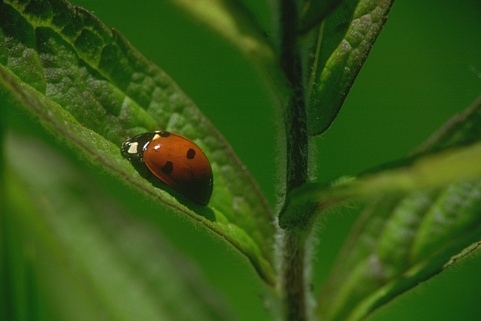
\includegraphics[width=\linewidth]{segmentation/entradas-posta/mariquita}
		\caption{Entrada}
	\end{subfigure}
	\begin{subfigure}{0.4\linewidth}
		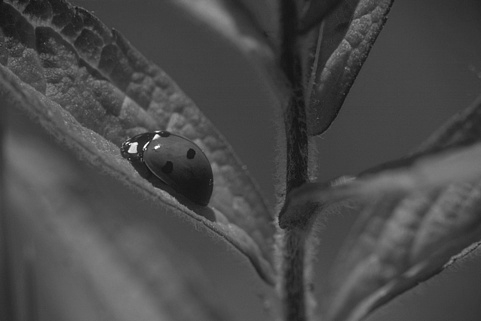
\includegraphics[width=\linewidth]{segmentation/informe/mariquita}
		\caption{Entrada en escala de grises}
	\end{subfigure}
	\begin{subfigure}{0.4\linewidth}
		\includegraphics[width=\linewidth]{segmentation/salidas/{0.0.mariquita.jpg.6000.-1}.png}
		\caption{$\sigma = 0,\ k = 6000$}
	\end{subfigure}
	\begin{subfigure}{0.4\linewidth}
		\includegraphics[width=\linewidth]{segmentation/salidas/{0.0.mariquita.jpg.600.1000}.png}
		\caption{$\sigma = 0,\ k = 600,\ g = 1000$}
	\end{subfigure}
	\caption{Distintas configuraciones, aquellas que no especifican valores
	para $g$ no tuvieron paso de simplificación.}
\end{figure}

Dado que la evidente similaridad de color no se traslada a la entrada en escala
de grises. El algorimo no puede construir un segmento coherente para las
hojas\footnote{El insecto tiene su propio segmento pero el color es demasiado
similar por lo que no puede apreciarse bien}.

Aún así esta es una deficiencia clara de la técnica las hojas muestra una de
las texturas en las que el algoritmo de segmentación fallan. También puede
notarse que para tener una segmentación ``\emph{pasable}'' se requirió de un
valor de $k$ muy alto comparado con los anteriormente utilizados (6000).

\subsubsection{Grano y halo}

La importancia del desenfoque no es evidente en todas las imágenes, la
siguiente escena muestra un defecto que ocurre cuando las fotos tienen mucho
grano (y un defecto que ocurre al desenfocar mucho):

\begin{figure}[h]
	\centering
	\begin{subfigure}{0.3\linewidth}
		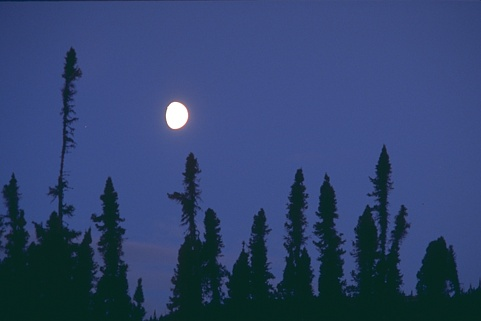
\includegraphics[width=\linewidth]{segmentation/entradas-posta/noche}
		\caption{Entrada}
	\end{subfigure}
	\begin{subfigure}{0.3\linewidth}
		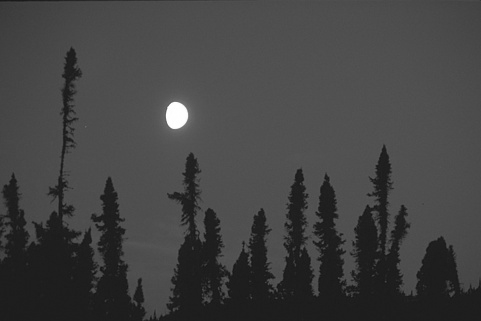
\includegraphics[width=\linewidth]{segmentation/informe/noche}
		\caption{Escala de grises}
	\end{subfigure}
	\begin{subfigure}{0.3\linewidth}
		\includegraphics[width=\linewidth]{segmentation/salidas/{0.0.noche.jpg.600.-1}.png}
		\caption{$\sigma = 0,\ k = 600$}
	\end{subfigure}
	\begin{subfigure}{0.3\linewidth}
		\includegraphics[width=\linewidth]{segmentation/salidas/{0.2.noche.jpg.600.-1}.png}
		\caption{$\sigma = 0.2,\ k = 0$}
	\end{subfigure}
	\begin{subfigure}{0.3\linewidth}
		\includegraphics[width=\linewidth]{segmentation/salidas/{0.4.noche.jpg.600.-1}.png}
		\caption{$\sigma = 0.4,\ k = 600$}
	\end{subfigure}
	\begin{subfigure}{0.3\linewidth}
		\includegraphics[width=\linewidth]{segmentation/salidas/{0.6.noche.jpg.600.-1}.png}
		\caption{$\sigma = 0.6,\ k = 600$}
	\end{subfigure}
	\begin{subfigure}{0.4\linewidth}
		\includegraphics[width=\linewidth]{segmentation/salidas/{0.8.noche.jpg.600.-1}.png}
		\caption{$\sigma = 0.8,\ k = 600$}
	\end{subfigure}
	\begin{subfigure}{0.4\linewidth}
		\includegraphics[width=\linewidth]{segmentation/salidas/{1.0.noche.jpg.600.-1}.png}
		\caption{$\sigma = 1,\ k = 600$}
	\end{subfigure}
	\caption{Segmentación de una escena simple con grano.}
\end{figure}

El defecto causado por el grano ocurre por la misma razón que se segmenta en 3
partes la imagen de prueba (degradé, negro y ruido) antes discutida. El
algoritmo construye las regiones de acuerdo a la similaridad entre sus
componentes, agrupando los píxeles que más se parecen entre sí primero. Cómo
esto genera componentes grandes el factor de juego que aporta $\tau(e)$ se
reduce lo suficiente como para que regiones muy similares no se unan una vez
que el algoritmo comienza a procesar las aristas con mayor diferencia propias
del grano.

El defecto del halo (el que puede verse en g y h) es uno causado por desenfoque
excesivo. Aquí entra en juego el mismo factor pero sobre la interfaz que se
forma en el límite entre dos regiones. Una forma de contrarestarlo es
utilizando el posprocesamiento greedy que unirá estos segmentos por su eje de
menor peso si son suficientemente pequeños.

\subsubsection{Simplificación greedy}

Una vez segmentada una imagen el algoritmo arroja comúnmente pequeños segmentos
de pocos píxeles. Es por esto que se implementó el proceso de simplificación
greedy, que suponiendo que el eje más liviano es el punto más obvio en el que
unir dos regiones intenta simplificar la segmentación eliminando detalles
menores.

\begin{figure}[h]
	\centering
	\begin{subfigure}{0.3\linewidth}
		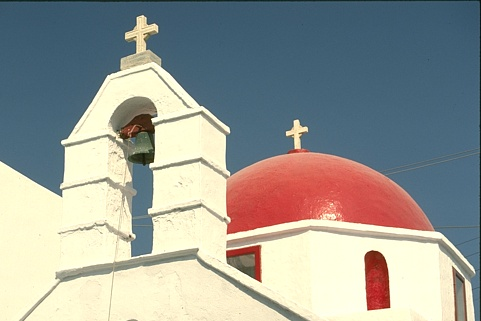
\includegraphics[width=\linewidth]{segmentation/entradas-posta/iglesia}
		\caption{Entrada}
	\end{subfigure}
	\begin{subfigure}{0.3\linewidth}
		\includegraphics[width=\linewidth]{segmentation/salidas/{0.8.iglesia.jpg.600.-1}.png}
		\caption{$\sigma = 0.8,\ k = 600$}
	\end{subfigure}
	\begin{subfigure}{0.3\linewidth}
		\includegraphics[width=\linewidth]{segmentation/salidas/{0.8.iglesia.jpg.600.1000}.png}
		\caption{$g = 1000$}
	\end{subfigure}
	\caption{Segmentacion de \texttt{iglesia.jpg}}
\end{figure}

En esta imagen (y la siguiente) pueden notarse pequeñas regiones de pocos
píxeles que se eliminan al correr el proceso de simplificación. Entregando una
segmentación más simple que podría servir de entrada a otro algoritmo
(dividiendo la imagen original en estos segmentos, por ejemplo).

\newpage

\begin{figure}[h]
	\centering
	\begin{subfigure}{0.3\linewidth}
		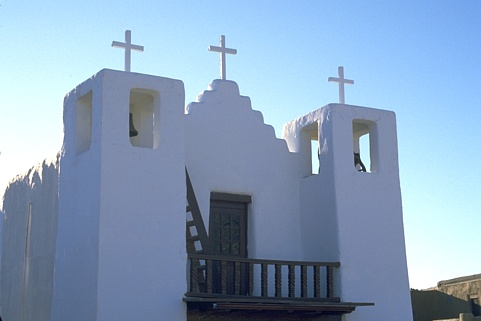
\includegraphics[width=\linewidth]{segmentation/entradas-posta/iglesia_2}
		\caption{Entrada}
	\end{subfigure}
	\begin{subfigure}{0.3\linewidth}
		\includegraphics[width=\linewidth]{segmentation/salidas/{0.8.iglesia_2.jpg.600.-1}.png}
		\caption{$\sigma = 0.8,\ k = 600$}
	\end{subfigure}
	\begin{subfigure}{0.3\linewidth}
		\includegraphics[width=\linewidth]{segmentation/salidas/{0.8.iglesia_2.jpg.600.1000}.png}
		\caption{$g = 1000$}
	\end{subfigure}
	\caption{Segmentacion de \texttt{iglesia\_2.jpg}}
\end{figure}

En esta imagen puede observarse uno de los defectos de la simplificación
greedy.  Sobre la escalera se construyeron segmentos correspondientes al
espacio entre peldaños, pero estos se vieron simplificados en pos de reducir la
cantidad de segmentos de la imagen. Otro ejemplo de imagen en la cuál ocurre
esto es en \texttt{ciudad.jpg}\footnote{Puede verse al segmentar esta imagen
que se generan segmentos indeseables de mayor tamaño que las ventanas de los
edificios.} Cómo el proceso de simplificación sólo tiene en cuenta el tamaño de
las regiones este defecto no es siempre corregible cambiando el valor de $g$.

\subsubsection{Análisis de los videos adjuntos}

Adjunto a este trabajo se encuentran tres vídeos dónde se varían $k$, $g$ y
$\sigma$ en \texttt{autitos.jpg}.

Al variar $g$ puede verse que muchos de los valores no representan cambio
alguno pero los cambios generan refinaciones de la misma segmentación por lo
que consideramos que es un parámetros útil para generar segmentaciones con una
cantidad acotada de segmentos.

Al variar $k$ se nota cómo parte del ``ruido'' no se une nunca a los segmentos
más grandes (lo cuál fué la razón principal de escribir el postprocesamiento) y
cómo valores muy altos de $k$ eliminan detalles importantes (cómo el cartel de
castrol en el fondo o el número del auto en la competencia). Esto nos indica
que hay puntos dónde fijar $k$ y variar $g$ (para eliminar ruido) puede
producir mejores segmentaciones que simplemente aumentar $k$. Otra cosa notable
es que pasado un valor de $k$ los cambios se reducen muchísimo y la
segmentación se ``estabiliza''. Esta observación es interesante si se pretende
utilizar un programa para buscar una ``buena segmentación'' variando los
parámetros del algoritmo.

Variando $\sigma$ la imagen se degenera muy rápidamente generando halos y
``redondeando'' los bordes de las regiones. Esto nos muestra que el desenfoque
tiene un rango muy acotado de valores sobre los cuáles no afecta notablemente a
la imagen, lo cuál es de gran ayuda (por acotar la búsqueda) a la hora de
buscar una buena segmentación variando los parámetros. Sin embargo vale la pena
notar que el efecto del desenfoque es relativo al tamaño de la imagen (una
imagen muy grande requerirá un $\sigma$ más alto para mostrar estos
``artifacts'').

\clearpage
